\documentclass[a4paper,10pt]{article}
\input{/home/frr/UFSC/Pagina/Dropbox/Modelos/Modelo_prova_latex/estilo_prova.tex}

\begin{document}


\professor{Fábio Rodrigues de la Rocha}
\turma{06655}
\codigodisciplina{ARA7546}
\disciplina{Circuitos Digitais}
\data{24/03/2014}
\hlimite{20:20}
\listaexercicios{5}

\begin{center}
\large{\fbox{\mbox{Registradores}}}
\end{center}


\questao{A figura abaixo mostra dois latches SR ligados em cascata. Desenhe a onda esperada na saída  $Q_{2}$.}

\begin{figure}[H]
   \centering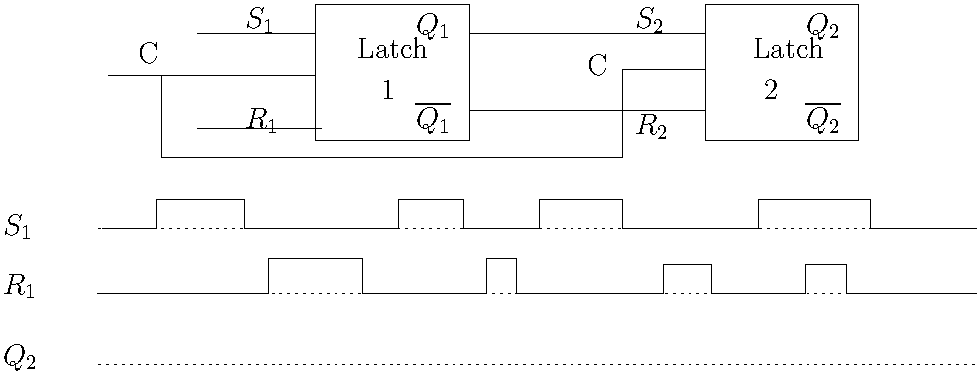
\includegraphics[width=0.5\textwidth]{latches}
\end{figure}

\questao{A figura anterior. Troque os latches por Flip-Flops e desenhe a onda esperada na saída  
$Q_{2}$.}

\questao{Assumindo que temos um Flip-Flip do tipo D, crie um circuito para convertê-lo em Flip-Flop JK.}

\questao{O diagrama abaixo utiliza os CI 74LS75 (Duplo Flip-Flop JK) e CI 74LS112 (Duplo Latch D). Dada a configuração de entradas do diagrama e os sinais E,
D e Reset, desenhe os sinais Q0, J1, Q1}

\begin{figure}[H]
   \centering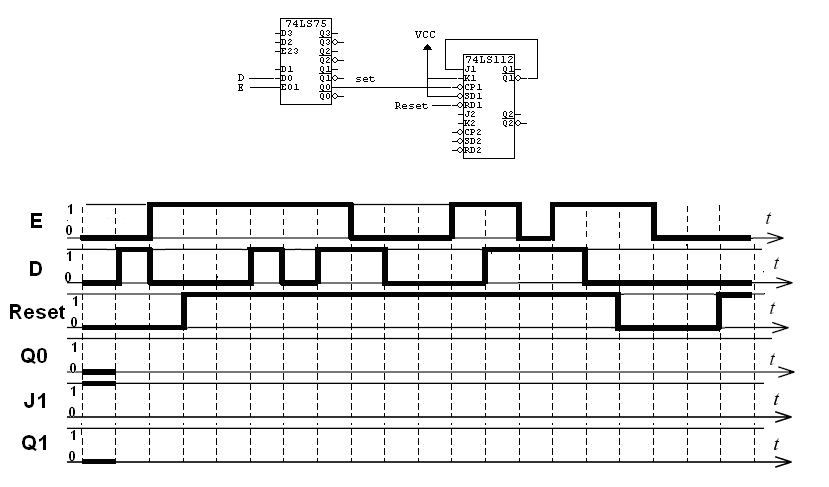
\includegraphics[width=0.6\textwidth]{ondas}
\end{figure}

\questao{Apresente o circuito interno X para que o circuito mostrado na figura funcione corretamente.}

\begin{figure}[H]
   \centering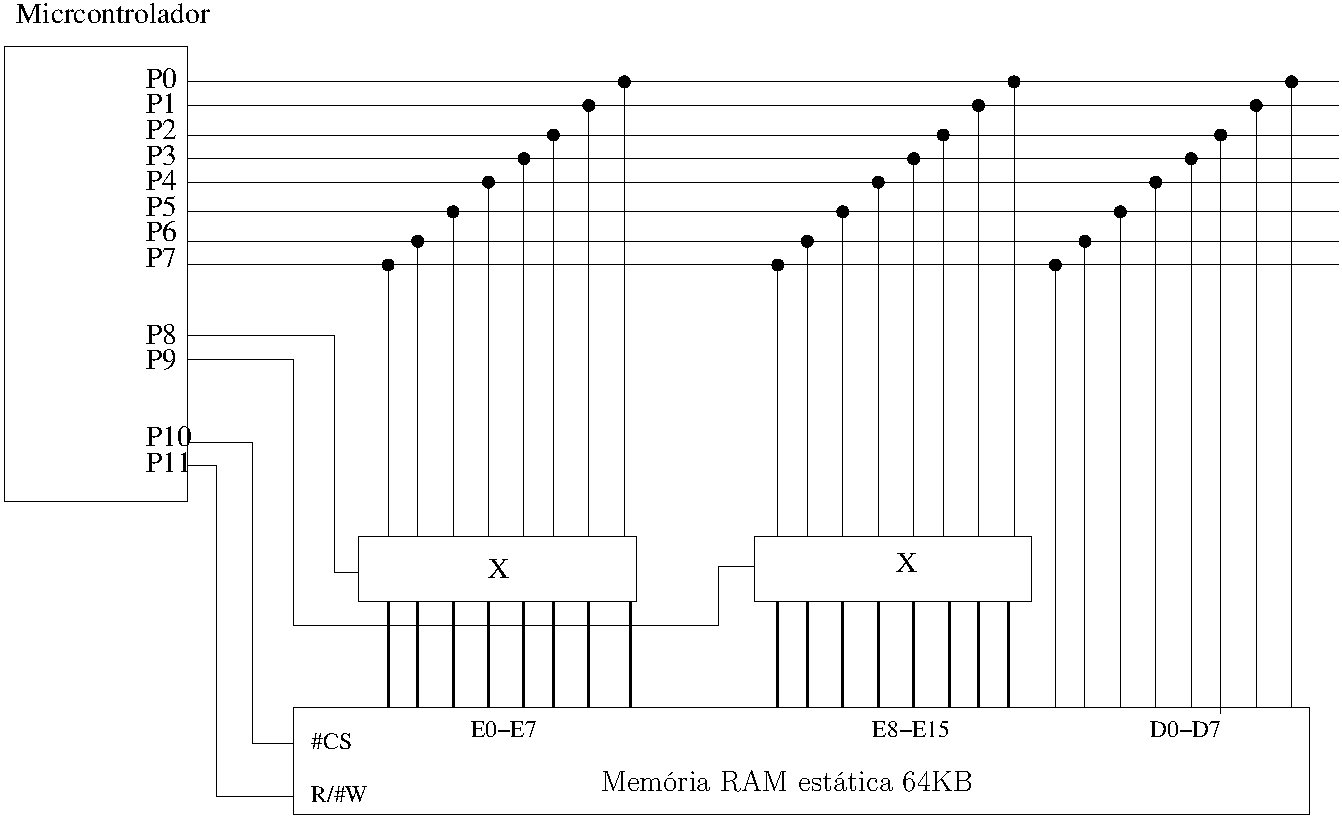
\includegraphics[width=0.7\textwidth]{acesso_memoria}
\end{figure}


\questao{Explique o funcionamento e função do circuito apresentado abaixo.}

\begin{figure}[H]
   \centering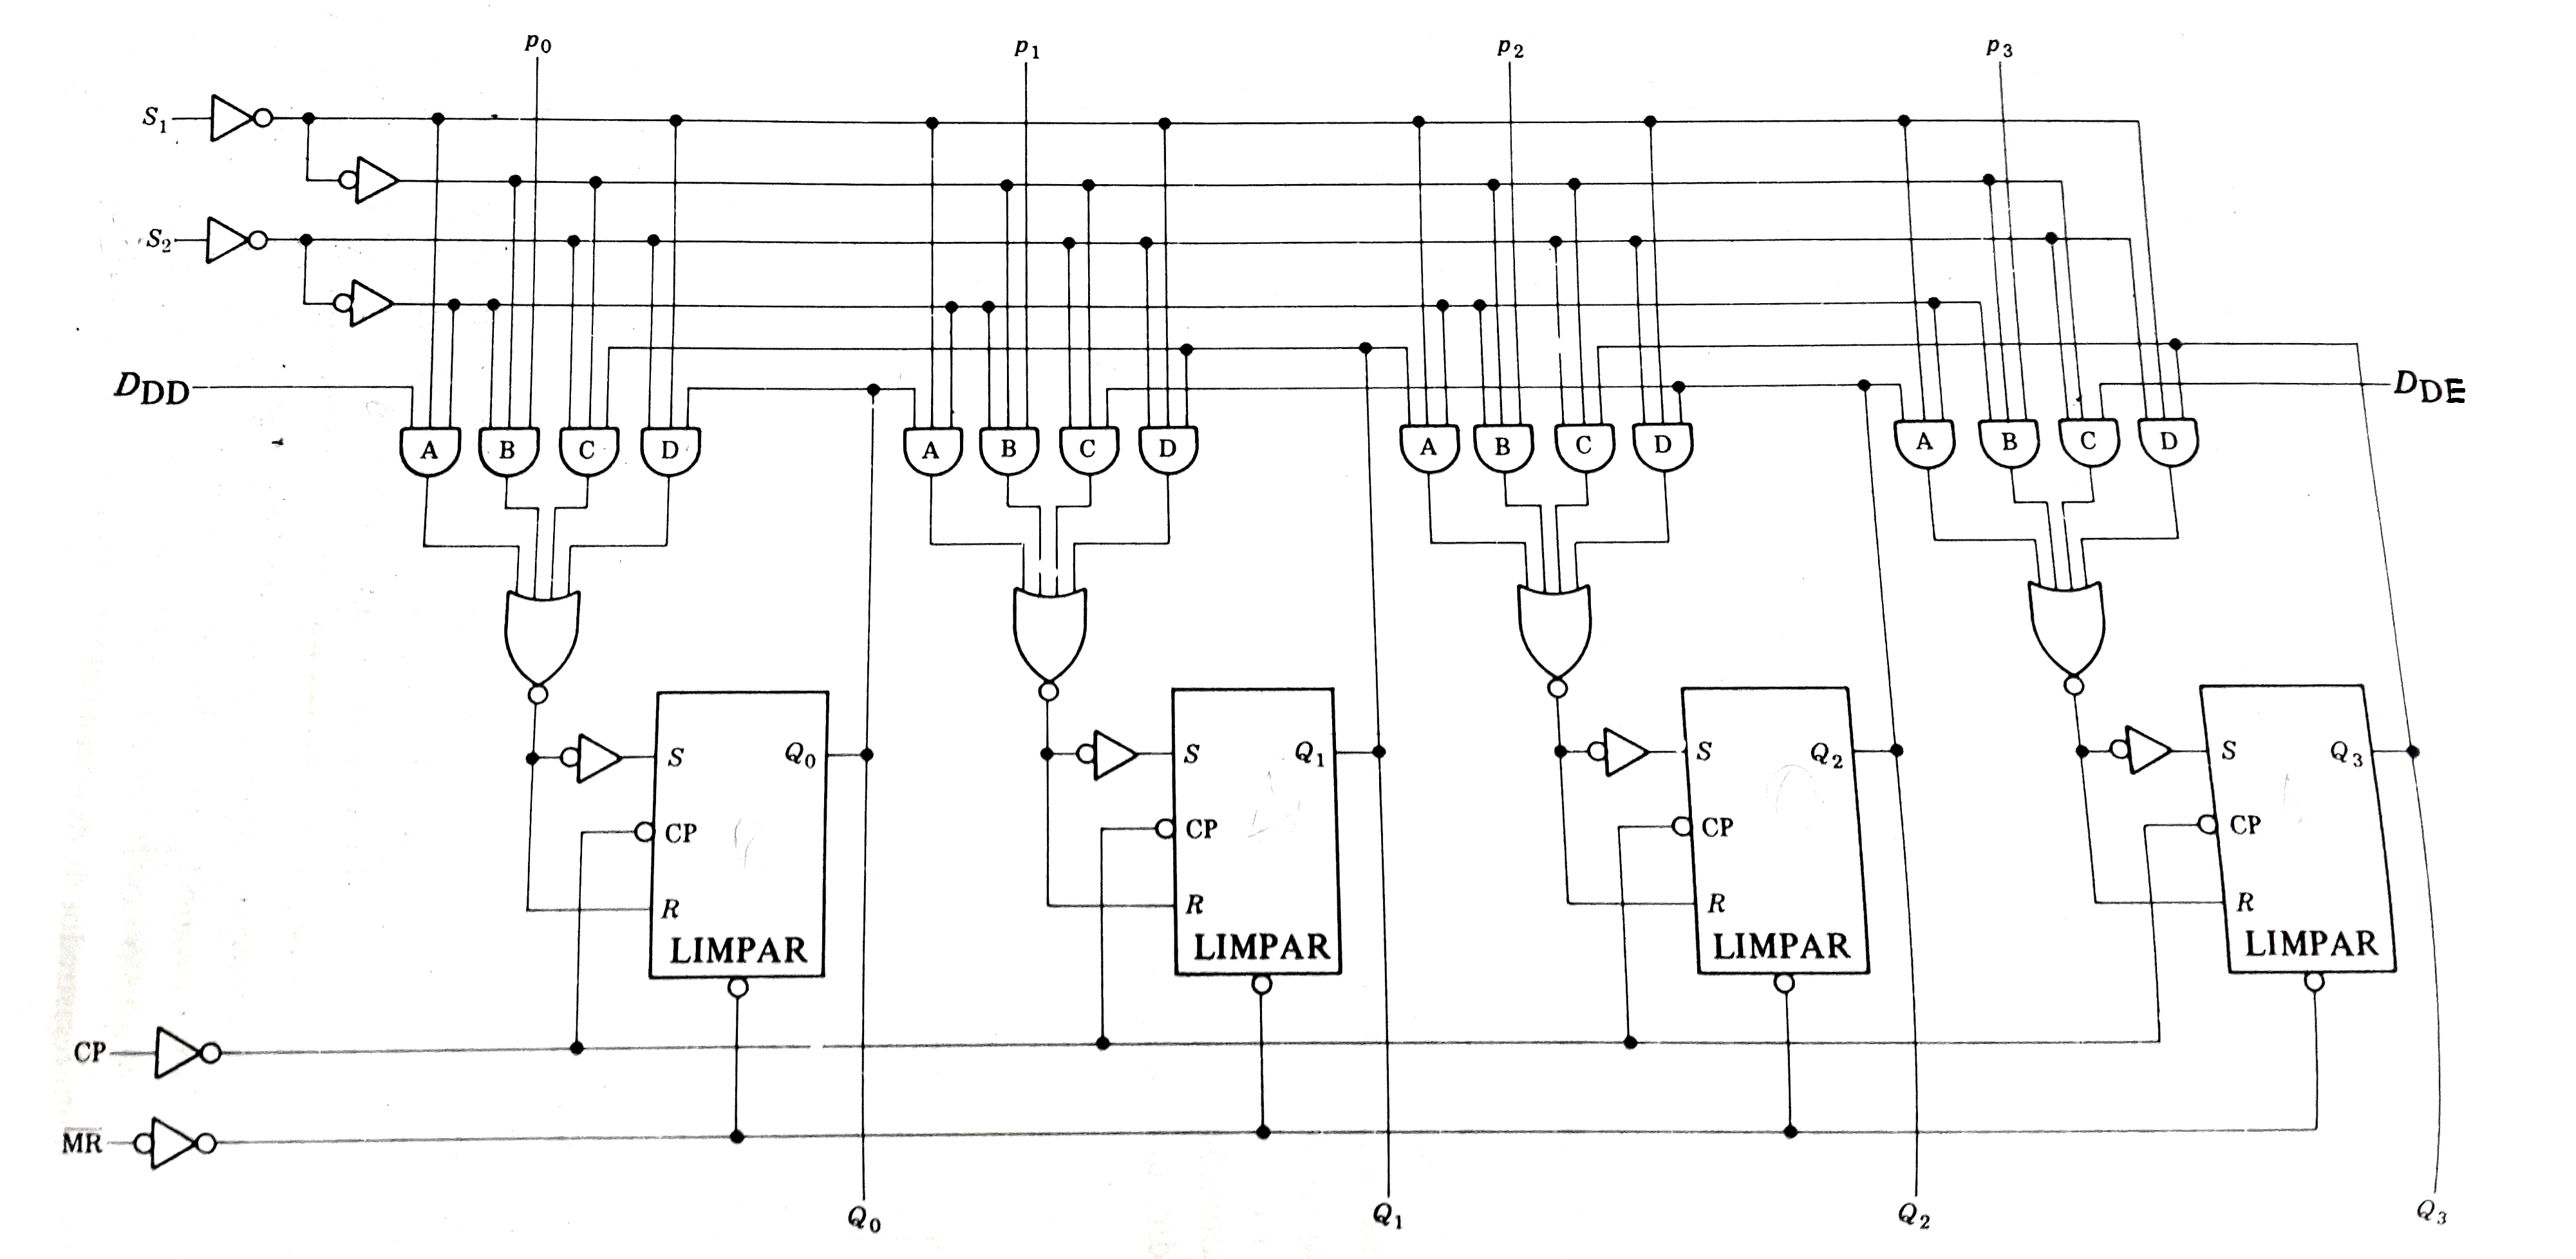
\includegraphics[width=0.7\textwidth]{Registrador_deslocamento_universal}
\end{figure}



\questao{Utilizando Flip-Flips do tipo D, crie um registrador de 4 bits onde os dados são entrados em série e ficam disponíveis em paralelo.}


%\begin{figure}[H]
%\begin{minipage}[b]{0.4\textwidth}
%\centering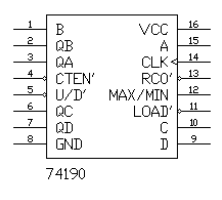
\includegraphics[width=0.6\textwidth]{74190}
%\end{minipage}
%\hspace{0.5cm}
%\begin{minipage}[b]{0.6\textwidth}
%\centering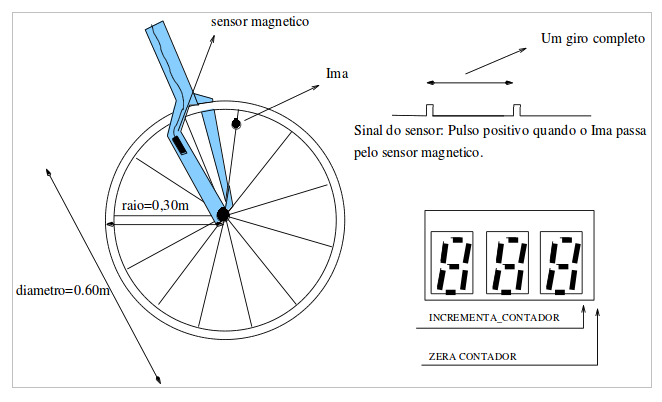
\includegraphics[width=0.6\textwidth]{bicicleta}
%\end{minipage}
%\end{figure}




\end{document}